\chapter{El camino hasta el sensor: atmósfera, Sol y superficie}\label{cap:atmosfera}

\objetivos{
\begin{itemize}
  \item Explicar qué es una ventana atmosférica y por qué los canales de fuego están donde
  están.
  \item Distinguir la radiación emitida de la radiación solar reflejada y decir en qué canal y
  a qué hora importa cada una.
  \item Identificar las tres situaciones que más engañan a un detector de fuego: nubes, brillo
  solar sobre agua y suelos calientes y reflectantes.
  \item Explicar por qué las detecciones nocturnas son más limpias que las diurnas.
\end{itemize}}

\section{La radiación no viaja sola}

En el capítulo anterior el fuego emitía y el sensor recibía, como si entre ambos hubiera vacío.
En realidad la radiación atraviesa toda la atmósfera, y en el camino le pueden pasar tres cosas
(figura~\ref{fig:camino}):

\begin{description}[leftmargin=1.2em]
  \item[Absorción.] Una molécula de gas captura la radiación y se queda con su energía.
  \item[Dispersión.] Una molécula o una partícula (humo, polvo, gotas) desvía la radiación en
  otra dirección, de modo que deja de ir hacia el sensor.
  \item[Emisión.] La propia atmósfera, que también está a cierta temperatura, emite radiación
  térmica que se suma a la señal.
\end{description}

Además, de día, el sensor no solo recibe lo que la superficie \emph{emite}, sino también la luz
del Sol que la superficie \emph{refleja}.

\begin{figure}[ht]
\centering
% Cuatro paneles: las etiquetas quedan fuera de las trayectorias.
\begin{tikzpicture}[font=\footnotesize,
  pics/sensor/.style={code={
    \fill[ceniza!45] (-.22,-.16) rectangle (.22,.16);
    \fill[cielo!75] (-.85,-.12) rectangle (-.30,.12);
    \fill[cielo!75] (.30,-.12) rectangle (.85,.12);
  }}]
  \foreach \x/\y in {0/0,7.7/0,0/-5.3,7.7/-5.3}{
    \fill[cieloClaro!80] (\x,\y+.5) rectangle ++(7,3);
    \fill[bosque!35] (\x,\y+.2) rectangle ++(7,.3);
  }
  \begin{scope}
    \node[anchor=west,font=\small\bfseries] at (0,4.5) {(a) Luz solar reflejada};
    \shade[inner color=yellow!70!white,outer color=brasa] (.8,3.85) circle (.32);
    \node[anchor=west] at (1.2,3.85) {Sol};
    \pic at (4.6,3.85) {sensor};
    \node[anchor=west] at (5.6,3.85) {sensor};
    \draw[->,very thick,brasa] (1,3.5)--(2.7,.57);
    \draw[->,very thick,brasa] (2.7,.57)--(4.5,3.58);
    \node[align=center] at (.85,2.0) {luz solar\\incidente};
    \node[align=left,anchor=west] at (4.1,1.8) {luz solar\\reflejada};
    \node at (3.5,-.08) {superficie};
  \end{scope}
  \begin{scope}[shift={(7.7,0)}]
    \node[anchor=west,font=\small\bfseries] at (0,4.5) {(b) Emisión del fuego y pérdidas};
    \pic at (1.3,3.85) {sensor};
    \node[anchor=west] at (2.3,3.85) {sensor};
    \shade[inner color=yellow,outer color=fuego] (1.3,.65) ellipse (.33 and .17);
    \draw[->,very thick,fuego] (1.3,.85)--(1.3,3.58);
    \node[anchor=west] at (1.6,3.15) {transmitida};
    \draw[thick,fuego] (1.3,1.45)--(3.7,2.55);
    \draw[thick,ceniza] (3.59,2.44)--(3.81,2.66) (3.59,2.66)--(3.81,2.44);
    \node[anchor=west] at (4,2.55) {absorción};
    \draw[->,thick,fuego,dashed] (1.3,1.2)--(3.7,1.55);
    \node[anchor=west] at (4,1.55) {dispersión};
    \node at (1.3,-.08) {fuego};
  \end{scope}
  \begin{scope}[shift={(0,-5.3)}]
    \node[anchor=west,font=\small\bfseries] at (0,4.5) {(c) Emisión de la atmósfera};
    \pic at (4.6,3.85) {sensor};
    \node[anchor=west] at (5.6,3.85) {sensor};
    \fill[cielo!25] (3.1,1.65) circle (.4);
    \fill[cielo] (3.1,1.65) circle (.065);
    \draw[->,very thick,cielo] (3.1,1.65)--(4.5,3.58);
    \node[align=left,anchor=west] at (.35,2.55) {emisión térmica\\de la atmósfera};
    \node at (3.5,-.08) {superficie};
  \end{scope}
  \begin{scope}[shift={(7.7,-5.3)}]
    \node[anchor=west,font=\small\bfseries] at (0,4.5) {(d) Fuego oculto por una nube};
    \pic at (4.6,3.85) {sensor};
    \node[anchor=west] at (5.6,3.85) {sensor};
    \fill[white] (3.5,2.5) ellipse (1.25 and .48);
    \fill[white] (3.0,2.75) ellipse (.7 and .38);
    \fill[white] (4.1,2.75) ellipse (.8 and .4);
    \node[align=center] at (1.0,2.55) {nube\\opaca};
    \shade[inner color=yellow,outer color=fuego] (3.5,.65) ellipse (.33 and .17);
    \draw[->,very thick,fuego] (3.5,.85)--(3.5,2.03);
    \node[fuego,font=\small] at (3.5,2.17) {$\times$};
    \node[align=left,anchor=west] at (4.9,1.45) {no llega\\la señal\\del fuego};
    \node at (3.5,-.08) {fuego oculto};
  \end{scope}
\end{tikzpicture}

\caption{Cuatro procesos que modifican la señal del sensor. (a) La superficie refleja luz
solar. (b) Parte de la emisión del fuego llega al sensor; otra parte se absorbe o se dispersa.
(c) La atmósfera añade su propia emisión térmica. (d) Una nube opaca impide observar el
fuego situado debajo. Los paneles separan los procesos para explicarlos; en una escena
real pueden ocurrir simultáneamente.}
\label{fig:camino}
\end{figure}

\section{Transmitancia y ventanas atmosféricas}

\begin{definicion}{transmitancia}
La transmitancia atmosférica $\tau_\lambda$ es la fracción de la radiación de longitud de onda
$\lambda$ que logra atravesar la atmósfera sin ser absorbida ni dispersada. Vale 1 si la
atmósfera es perfectamente transparente y 0 si es totalmente opaca.
\end{definicion}

Los gases de la atmósfera absorben de forma muy selectiva. El vapor de agua, el dióxido de
carbono y el ozono tienen bandas de absorción intensas en longitudes de onda concretas, y entre
ellas quedan intervalos donde la atmósfera es casi transparente. Esos intervalos se llaman
\termino{ventanas atmosféricas}, y son los únicos por los que un satélite puede ver la
superficie (figura~\ref{fig:ventanas}).

\begin{figure}[ht]
\centering
\begin{tikzpicture}
\begin{axis}[width=13.5cm,height=6.2cm,xmin=1,xmax=14,ymin=0,ymax=1.08,
  xlabel={Longitud de onda (\um)},ylabel={Transmitancia $\tau$},
  xtick={1,2,3,4,5,6,7,8,9,10,11,12,13,14},axis lines*=left,
  ytick={0,0.5,1},yticklabels={0,{0,5},1}]
\addplot[fill=cielo!30,draw=cielo,thick,smooth] coordinates {
 (1,0.86)(1.25,0.9)(1.33,0.35)(1.38,0.02)(1.44,0.3)(1.55,0.9)(1.7,0.9)(1.8,0.25)(1.9,0.02)
 (1.98,0.4)(2.1,0.88)(2.3,0.88)(2.5,0.3)(2.6,0.02)(2.8,0.02)(2.95,0.2)(3.2,0.55)(3.5,0.85)
 (3.75,0.9)(3.95,0.92)(4.1,0.75)(4.2,0.05)(4.3,0.01)(4.45,0.1)(4.6,0.6)(4.8,0.7)(5.0,0.5)
 (5.3,0.1)(5.6,0.01)(7.0,0.01)(7.5,0.1)(7.9,0.5)(8.3,0.78)(9.0,0.85)(9.4,0.55)(9.6,0.3)
 (9.8,0.6)(10.2,0.88)(11,0.9)(12,0.86)(12.6,0.7)(13.2,0.4)(14,0.08)} \closedcycle;
\draw[fuego,very thick] (axis cs:3.96,0)--(axis cs:3.96,1.02);
\draw[fuego,very thick] (axis cs:11,0)--(axis cs:11,1.02);
\node[font=\footnotesize,fuego,anchor=south] at (axis cs:3.96,1.0) {4~\um};
\node[font=\footnotesize,fuego,anchor=south] at (axis cs:11,1.0) {11~\um};
\node[font=\footnotesize,ceniza] at (axis cs:2.7,0.16) {H$_2$O};
\node[font=\footnotesize,ceniza] at (axis cs:4.3,0.2) {CO$_2$};
\node[font=\footnotesize,ceniza] at (axis cs:6.3,0.12) {H$_2$O};
\node[font=\footnotesize,ceniza] at (axis cs:9.6,0.17) {O$_3$};
\node[font=\footnotesize,ceniza] at (axis cs:13.7,0.3) {CO$_2$};
\end{axis}
\end{tikzpicture}
\caption{Esquema de la transmitancia de la atmósfera en el infrarrojo (curva simplificada, no
un cálculo exacto). Las zonas altas son ventanas; las hondonadas llevan el nombre del gas que
absorbe. Los dos canales de fuego caen dentro de ventanas.}
\label{fig:ventanas}
\end{figure}

Las dos ventanas que nos interesan son la del \textbf{infrarrojo medio}, entre 3,5 y 4~\um{}
aproximadamente, y la del \textbf{infrarrojo térmico}, entre 8 y 12,5~\um{} (interrumpida por
el ozono cerca de 9,6~\um). La ventana media limita por la derecha con una banda de absorción
muy fuerte del CO$_2$ centrada en 4,3~\um. Por eso los canales de fuego se sitúan justo antes:
3,96~\um{} en MODIS y 3,74~\um{} en la banda I4 de VIIRS.

Incluso dentro de una ventana, la transmitancia no es 1. El sensor recibe aproximadamente
\begin{equation}\label{eq:transferencia}
  L_{\text{sensor}} \;\approx\; \tau_\lambda\, L_{\text{superficie}} \;+\; L_{\text{atmósfera}},
\end{equation}
donde el primer término es la señal de la superficie atenuada y el segundo es la emisión de la
propia atmósfera. En una atmósfera húmeda (la selva, por ejemplo) $\tau$ baja y la atmósfera
emite más, mientras que en el aire seco y delgado de la sierra a más de 3000 metros la señal
llega más limpia. El efecto es moderado en estos canales, pero es una de las razones por las que
el rendimiento de la detección no es idéntico en todas las regiones.

\section{El humo}

Podría pensarse que el humo de un incendio impide verlo desde el espacio. En el visible es así:
una columna de humo denso es opaca al ojo. Pero las partículas de humo son muy pequeñas, con
tamaños típicos de décimas de micrómetro, y una partícula dispersa con eficacia solo la
radiación cuya longitud de onda es comparable a su tamaño o menor. Para la radiación de 4 y de
11~\um, mucho más larga, el humo es casi transparente.

Esta es una de las grandes ventajas de detectar fuego en el infrarrojo: \textbf{se ve a través
del humo}. La excepción son las columnas de humo extremadamente densas de los incendios más
intensos, que sí pueden atenuar la señal y que motivaron ajustes específicos en la versión
actual del algoritmo de MODIS.

\section{Las nubes}

Las nubes son otra historia. Sus gotas y cristales de hielo miden entre unos pocos y decenas de
micrómetros, tamaños comparables a las longitudes de onda de nuestros canales, y absorben y
dispersan con mucha eficacia. Una nube espesa es \textbf{opaca} tanto a 4 como a 11~\um.

\begin{atencion}[Las nubes ocultan el fuego]
Si hay una nube espesa entre el fuego y el satélite, el fuego no se detecta. No aparece como
<<dudoso>> ni con baja confianza: simplemente no aparece. Los datos de focos no distinguen entre
<<no había fuego>> y <<no se pudo ver>>.
\end{atencion}

Esto introduce un sesgo sistemático que conviene tener presente desde ahora. En una región
donde la temporada de quemas coincide con cielos despejados (la estación seca de la sierra), la
mayoría de los fuegos tiene oportunidad de ser observada. En una región nubosa buena parte de la
actividad pasa inadvertida. La imagen real del capítulo~\ref{cap:modisviirs} muestra cuánta
superficie del centro del Perú puede estar cubierta en un día cualquiera de septiembre.

Las nubes, además, pueden generar falsas alarmas de día: son muy brillantes al reflejar el Sol,
también en 4~\um, y sus bordes crean contrastes fuertes entre píxeles vecinos. Por eso el primer
paso de todo algoritmo de fuego es construir una \termino{máscara de nubes} y descartar esos
píxeles antes de buscar fuego.

\section{El Sol entra en escena}

Hasta aquí la radiación venía de la superficie por estar caliente. De día hay una segunda
fuente: el Sol. La superficie refleja parte de la luz solar que recibe, y esa luz reflejada
también llega al sensor.

¿Cuánto importa? Depende del canal. El Sol es un cuerpo negro a unos 5800~K, y su emisión, muy
intensa en el visible, cae rápidamente hacia el infrarrojo. La emisión del suelo a 300~K hace lo
contrario: es despreciable en el visible y crece hacia el infrarrojo térmico. Las dos curvas se
cruzan justamente en la región del infrarrojo medio (figura~\ref{fig:cruce}).

\begin{figure}[ht]
\centering
\begin{tikzpicture}
\begin{axis}[width=13cm,height=7cm,xmode=log,ymode=log,xmin=0.4,xmax=20,ymin=0.01,ymax=300,
  xlabel={Longitud de onda (\um)},
  ylabel={Radiancia que sale de la superficie (\si{\watt\per\square\metre\per\steradian\per\micro\metre})},
  ylabel style={font=\small},
  xtick={0.5,1,2,4,11,20},xticklabels={{0,5},1,2,4,11,20},
  legend style={at={(0.5,0.05)},anchor=south,font=\small,draw=ceniza!40},
  grid=major,grid style={ceniza!15},samples=140,
  declare function={planck(\l,\T)=1.191e8/(\l^5*(exp(14388/(\l*\T))-1));}]
\addplot[brasa,very thick,domain=0.4:20] {0.15*6.8e-5*planck(x,5800)/3.1416*3.1416};
\addplot[cielo,very thick,domain=2.2:20] {planck(x,300)};
\legend{luz solar reflejada (reflectancia 0{,}15),emisión térmica del suelo a 300 K}
\draw[black,dashed,thick] (axis cs:3.96,0.01)--(axis cs:3.96,300);
\draw[black,dashed,thick] (axis cs:11,0.01)--(axis cs:11,300);
\node[font=\footnotesize,anchor=south west] at (axis cs:3.96,90) {4~\um};
\node[font=\footnotesize,anchor=south west] at (axis cs:11,90) {11~\um};
\end{axis}
\end{tikzpicture}
\caption{Luz solar reflejada frente a emisión térmica del suelo (orden de magnitud, con el Sol
alto y una superficie que refleja el 15\,{}\%). En el visible domina por completo la luz
reflejada; a 11~\um, la emisión. A 4~\um{} ambas son del mismo orden: es el único de los dos
canales de fuego al que el Sol afecta.}
\label{fig:cruce}
\end{figure}

La conclusión práctica es doble.

\textbf{A 11~\um{} el Sol es irrelevante.} Lo que mide ese canal es emisión térmica, de día y de
noche.

\textbf{A 4~\um{} el Sol sí cuenta.} De día, la radiancia de ese canal es la suma de la emisión
térmica y de una componente solar reflejada de magnitud comparable. Un píxel puede mostrar una
temperatura de brillo alta a 4~\um{} sin estar ardiendo, solo por ser muy reflectante.

\begin{definicion}{reflectancia}
La reflectancia $\rho$ de una superficie en un canal es la fracción de la radiación solar
incidente que refleja. Vale 0 para una superficie que no refleja nada y 1 para una que lo
refleja todo.
\end{definicion}

\section{Tres impostores}

Con lo anterior se pueden entender las tres situaciones clásicas en las que algo que no es fuego
se parece a un fuego.

\subsection{Brillo solar sobre el agua}

Una superficie de agua en calma actúa como un espejo. Si la geometría es la adecuada, es decir,
si el sensor queda en la dirección en la que el agua refleja el Sol, el píxel recibe un reflejo
directo e intensísimo. A esto se le llama \termino{sun glint} o brillo solar especular
(figura~\ref{fig:glint}). El reflejo es fuerte a 4~\um{} y casi nulo a 11~\um: la misma firma
que un fuego. Ocurre sobre mares, lagos, ríos anchos, arrozales inundados e incluso techos
metálicos.

\begin{figure}[ht]
\centering
\begin{tikzpicture}[scale=0.9]
  \fill[cielo!30] (0,0) rectangle (10,-0.5);
  \draw[cielo,thick] (0,0)--(10,0);
  \node[below,font=\footnotesize] at (5,-0.5) {superficie de agua en calma};
  \draw[dashed,ceniza] (5,0)--(5,4.2) node[above,font=\footnotesize]{vertical};
  \shade[inner color=yellow!80!white,outer color=brasa] (1.2,4.2) circle (0.42);
  \node[left,font=\footnotesize] at (0.75,4.2) {Sol};
  \draw[->,very thick,brasa] (1.5,3.9)--(4.95,0.05);
  \draw[->,very thick,brasa] (5.05,0.05)--(8.5,3.9);
  \fill[gray!45] (8.5,4.0) rectangle (9.2,4.45);
  \node[right,font=\footnotesize] at (9.3,4.2) {sensor};
  \draw (5,1.3) arc (90:132:1.3); \node[font=\footnotesize] at (4.5,1.65) {$\theta$};
  \draw (5,1.3) arc (90:48:1.3); \node[font=\footnotesize] at (5.5,1.65) {$\theta$};
\end{tikzpicture}
\caption{Geometría del brillo solar. Cuando el ángulo con que el sensor mira coincide con el
ángulo de reflexión del Sol, el agua devuelve un reflejo directo. Los algoritmos calculan este
ángulo para cada píxel y desconfían de las detecciones que caen cerca de esa condición.}
\label{fig:glint}
\end{figure}

\subsection{Suelos desnudos y calientes}

Un suelo seco y sin vegetación al mediodía reúne dos condiciones adversas: está realmente
caliente (puede superar los 320~K) y es bastante reflectante a 4~\um. Su temperatura de brillo a
4~\um{} es alta y la diferencia $\Delta T$ con el canal de 11~\um{} también. Los desiertos, las
zonas mineras a tajo abierto y los terrenos recién arados son candidatos a falsas alarmas.

\subsection{Bordes y contrastes}

Los algoritmos comparan cada píxel con sus vecinos. Allí donde el paisaje cambia bruscamente,
como una costa, la orilla de un lago, el borde de una nube o el límite entre bosque y un claro
recién abierto, el <<fondo>> con que se compara un píxel puede no representarlo bien, y una
diferencia normal del terreno se interpreta como anomalía térmica.

\section{Ver las bandas en una escena real de Perú}

La figura~\ref{fig:peru-bandas} muestra el mismo recuadro de la selva central peruana
en dos composiciones de VIIRS/Suomi NPP. No es una simulación: son imágenes del
15 de septiembre de 2024 obtenidas con NASA Worldview.\fuente{worldview}\fuente{gibs}
La comparación sirve para ver por qué cambiar de bandas cambia la información visual,
sin cambiar el terreno observado.

\begin{figure}[ht]
\centering
\begin{subfigure}[t]{.485\textwidth}
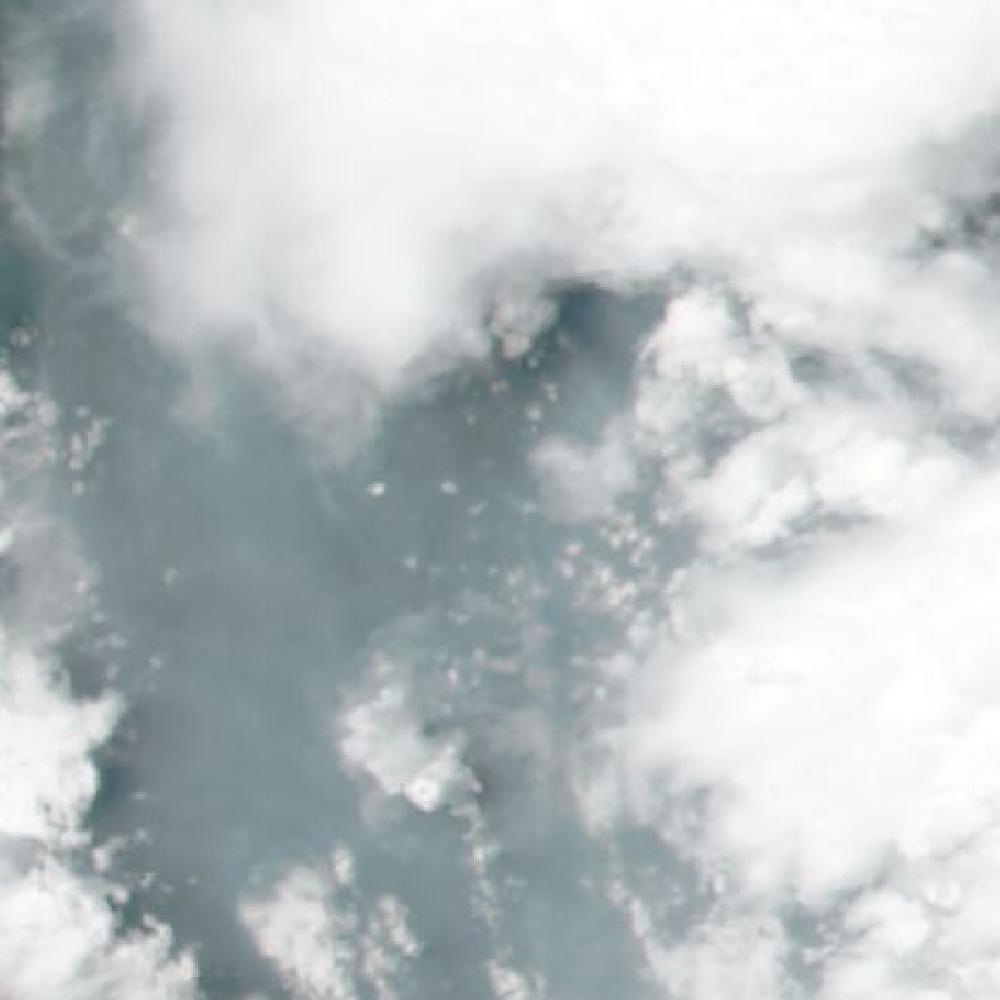
\includegraphics[width=\linewidth]{figuras/peru_selva_color.jpg}
\caption{Color verdadero: contraste visible y velo atmosférico.}
\end{subfigure}\hfill
\begin{subfigure}[t]{.485\textwidth}
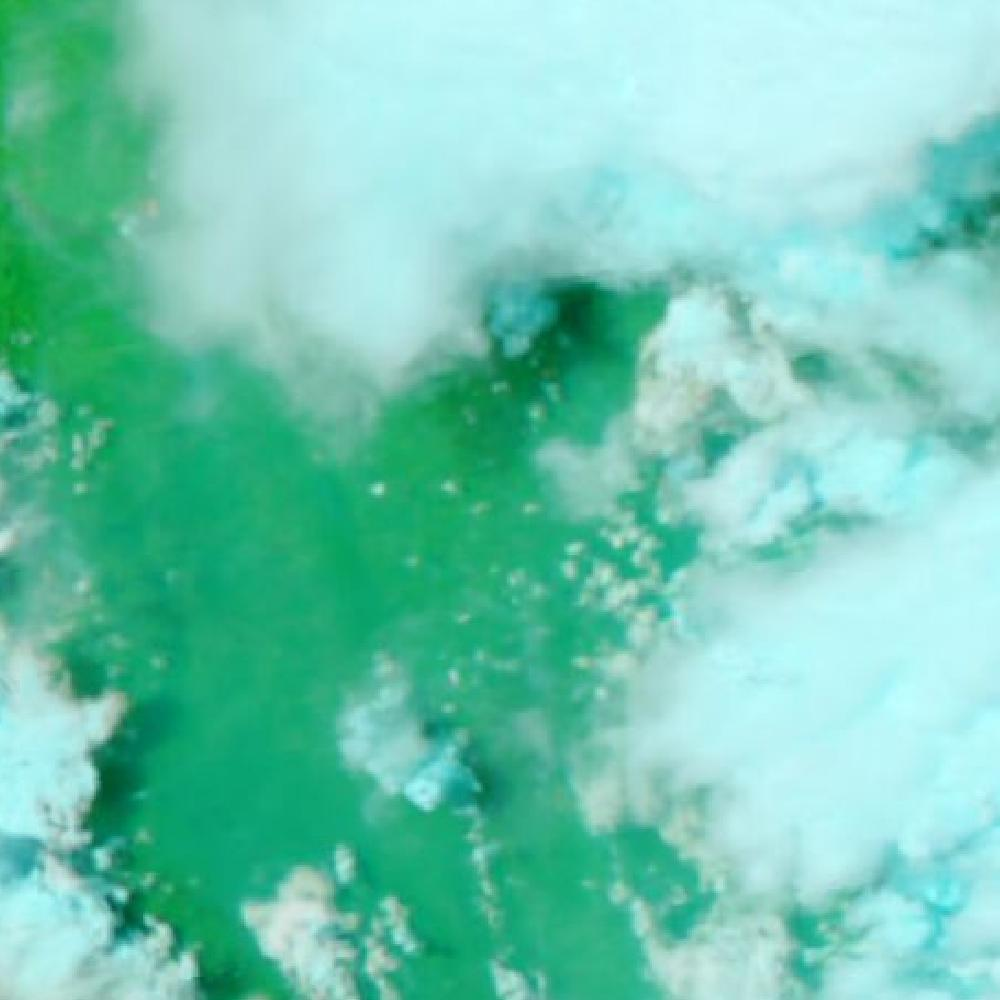
\includegraphics[width=\linewidth]{figuras/peru_selva_infrarrojo.jpg}
\caption{M11--I2--I1: otra respuesta espectral de la misma escena.}
\end{subfigure}
\caption{\textbf{Imágenes reales de Perú.} VIIRS/Suomi NPP, 15 de septiembre de 2024;
$10{,}5$--$9{,}5^\circ$ S, $75{,}5$--$74{,}5^\circ$ O, norte arriba. El recuadro mide
aproximadamente 111 km de norte a sur. Fuente: NASA GIBS/Worldview. Las manchas blancas
extensas siguen ocultando terreno; el cambio de colores no recupera esa información.}
\label{fig:peru-bandas}
\end{figure}

Observa primero la masa blanca de la parte superior y el borde derecho: no desaparece
en la composición infrarroja. Después compara la zona central: su contraste con el velo
gris cambia y la vegetación aparece verde en la composición M11--I2--I1. Ese verde es
una asignación de bandas a la pantalla, no una medición directa de salud vegetal.
Tampoco el velo permite diagnosticar su composición únicamente por este JPEG.

Esta pareja no se eligió para dibujar un contorno de incendio, sino para mostrar una
limitación: aun con bandas más informativas hay suelo que no vemos. El caso del
Camp Fire del capítulo~\ref{cap:problema} complementa la explicación al mostrar un
frente térmico visible y su transformación en puntos. En ambos casos, el pie de
imagen permite distinguir observación, representación e interpretación.

\section{El día y la noche}

De noche no hay Sol. Desaparece la componente reflejada a 4~\um, desaparece el brillo solar y
los suelos se han enfriado. La escena es más simple: todo lo que llega al sensor es emisión
térmica, y un píxel con exceso a 4~\um{} casi con seguridad contiene algo caliente de verdad.

Por eso los algoritmos usan umbrales \emph{distintos} de día y de noche, y por eso las
detecciones nocturnas tienen menos falsas alarmas. Los datos lo registran en la columna
\texttt{daynight}, con valores \texttt{D} y \texttt{N}.

Pero la noche tiene su propia trampa: el fuego también cambia. La mayoría de los incendios de
vegetación tiene un ciclo diario muy marcado, con máxima actividad a primera hora de la tarde,
cuando el aire está más caliente y seco y hay más viento, y mínima de madrugada. Muchas quemas
agrícolas se encienden por la mañana y están apagadas antes del anochecer. De noche se ve mejor,
pero hay menos que ver. El capítulo~\ref{cap:orbitas} retoma esta idea al hablar de la hora a la
que pasa cada satélite.

\begin{parareto}
La columna \texttt{daynight} permite separar detecciones diurnas y nocturnas. Para un calendario
de quemas agrícolas, las diurnas son las que capturan la actividad; las nocturnas señalan sobre
todo incendios que siguieron ardiendo sin control. Tratarlas por separado es una decisión de
diseño razonable y fácil de justificar.
\end{parareto}

\resumen

\begin{itemize}
  \item La atmósfera absorbe, dispersa y emite. Solo en las \textbf{ventanas atmosféricas} es
  suficientemente transparente; los canales de fuego están en la ventana de 3,5--4~\um{} y en
  la de 8--12,5~\um.
  \item El \textbf{humo} es casi transparente en el infrarrojo; las \textbf{nubes} espesas son
  opacas y ocultan el fuego sin dejar rastro en los datos.
  \item De día, el canal de 4~\um{} recibe emisión térmica \emph{y} luz solar reflejada en
  cantidades comparables; el de 11~\um{} solo emisión.
  \item Los principales impostores diurnos son el \textbf{brillo solar} sobre agua, los
  \textbf{suelos desnudos calientes} y los \textbf{bordes} de contraste.
  \item De noche la escena es más limpia y hay menos falsas alarmas, pero también menos fuego
  activo.
\end{itemize}

\ejercicios

\begin{enumerate}
  \item ¿Por qué no se coloca un canal de detección de fuego en 4,3~\um, donde las llamas emiten
  intensamente? Usa la figura~\ref{fig:ventanas}.
  \item Un píxel se observa a través de una atmósfera con $\tau = 0{,}85$ y la atmósfera aporta
  una radiancia propia de 0,05 unidades. Si la superficie emite 0,80 unidades, ¿qué radiancia
  llega al sensor según la ecuación~\eqref{eq:transferencia}? ¿Es mayor o menor que la que
  salió de la superficie?
  \item Explica por qué un incendio bajo una capa de humo espeso sí puede detectarse y uno bajo
  una nube espesa no.
  \item Un lago de la sierra aparece una tarde como una hilera de focos de baja confianza.
  Propón la explicación más probable y qué columna de los datos revisarías para apoyarla.
  \item Una región tiene su temporada de quemas en plena estación de lluvias, con el cielo
  cubierto la mitad de los días. ¿El conteo de focos subestima o sobrestima la actividad real?
  ¿Afecta esto por igual a MODIS y a VIIRS?
  \item Da dos razones por las que una detección nocturna es más fiable que una diurna y una
  razón por la que, pese a ello, un registro solo nocturno sería un mal calendario de quemas
  agrícolas.
\end{enumerate}
